\chapter{Research Approach}
\label{chap:research}

\section{Research Purpose}
%The purpose of this study is to evaluate the suitability of polyglot persistence for management of evolving historical data.

The purpose of this study is to identify and evaluate solutions for management of historical data in continuous integration systems. Specifically, to evaluate the suitability of polyglot persistence (forward ref to pp) in that context.

\section{Research Questions}
RQ1: What are the challenges of monotonic data growth in continuous integration systems? \\
RQ2: How can historical data in continuous integration systems be managed in the long term? \\
RQ3: Does the value gained from solving the problem of monotonic growth in continuous integration systems outweigh the identified costs related to implementing a solution for the problem? \\

%RQ2.1: How effective is polyglot persistence using NoSQL? \\
%RQ2.2: How effective is a relational approach? \\

%Old questions\\
%RQ1: What are the main challenges when designing and implementing a polyglot persistence solution?\\
%RQ2: What solutions are feasible in the given context?\\
%RQ2.1: How does the solution handle structural variation on incoming data?\\
%RQ2.2: How does the solution address scalability?\\
%\\
%Draft for new Research Questions:\\
%How to handle the side effect of continuous integration?\\
%What are a feasible way of handling data from continous integration system in the long term?\\
%
%Continuous integration, data growth, challenges, benefits, possibilities\\
%The probem is unplanned data growth in the context of CI systems\\
%What is a better way to manage historical data in the long term?\\
%How in long term handle data in a continuous integration system?\\
%What is the current state of practise for management of historical data?\\

\section{Research Method}
This thesis will be conducted using design research methods based on knowledge from \cite{DS, Peffers, DesignEval}. Design research is performed by building and evaluating artifacts that are designed with the purpose of addressing a specified business need or problem \cite{DS}. 

%In design research, artifacts are designed and evaluated with the intention of solving important organizational problems \cite{DS}. "The goal of design-science research is utility" Skriv mer har 

Peffers et al.\ \cite{Peffers} describe an overall process for conducting design research which for the purposes of this thesis has been implemented as in figure~\ref{fig:peffer}. As can be noted in this figure, one important aspect of design research is its focus on iterative processes, where evaluation should inform reformulation of solution objectives and also give feedback to upcoming iterations of design and development. This part of Peffers process will be implemented by performing several iterations of design/development and demonstration/evaluation. If necessary, solution objectives can be changed as an increased understanding of the problem is gained. 

According to \cite{Peffers}, there are several possible entry points for a design research study. In our case the entry point is an objective-centered solution, since the need for the study originated from an industrial problem that could be addressed by constructing an artifact.
\begin{figure}[h!]
\centering
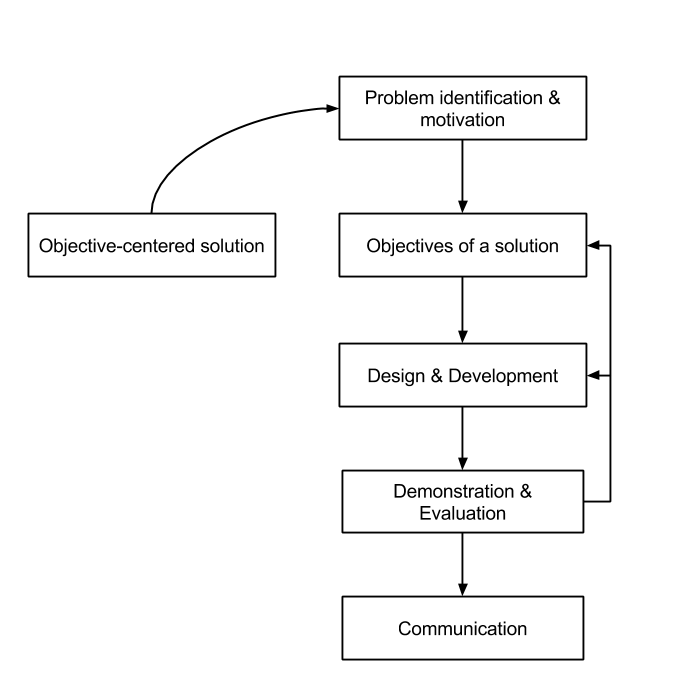
\includegraphics[width=0.7\pdfpagewidth]{figure/Peffer.png}
\caption{Peffers process}
\label{fig:peffer}
\end{figure}

In this thesis, our implementation of Peffers process laid out the overall framework used to design the study. First, we studied and defined the problem in more detail in collaboration with the CIMS development team. After this, we proceeded with the formulation of solution objectives which set the scope for this thesis. During this process, an overview of related work was written.

With solution objectives in place, work began on the two bigger phases, namely design/development and evaluation. In a given iteration of design/development, an artifact in the form of a prototype was either built from scratch or further developed.

For the evaluation process, options given by \cite{DesignEval} were used to define properties of the artifact, its purpose and actual approaches used for evaluation. The choices made can be seen in figure~\ref{fig:matrix}.

Further explanations of some of these choices are warranted;\\
The goal of the evaluation is to gather knowledge about the problem and its domain so as to put upcoming decisions made at Ericsson on a rational basis. As such, evaluation goes in line with the knowledge function described in \cite{DesignEval}.

A prototype solution was requested by stakeholders at Ericsson which is why the choice was made to evaluate using this method. Since we evaluate a prototype it is the artifact itself that is evaluated as opposed to the construction of the artifact.

Given that the thesis was conducted in collaboration with Ericsson, the artifact was evaluated in an organisational context and as such against the real world. Finally, we chose to do evaluation after the construction (ex post) of the artifact.

\begin{figure}[h!]
\centering
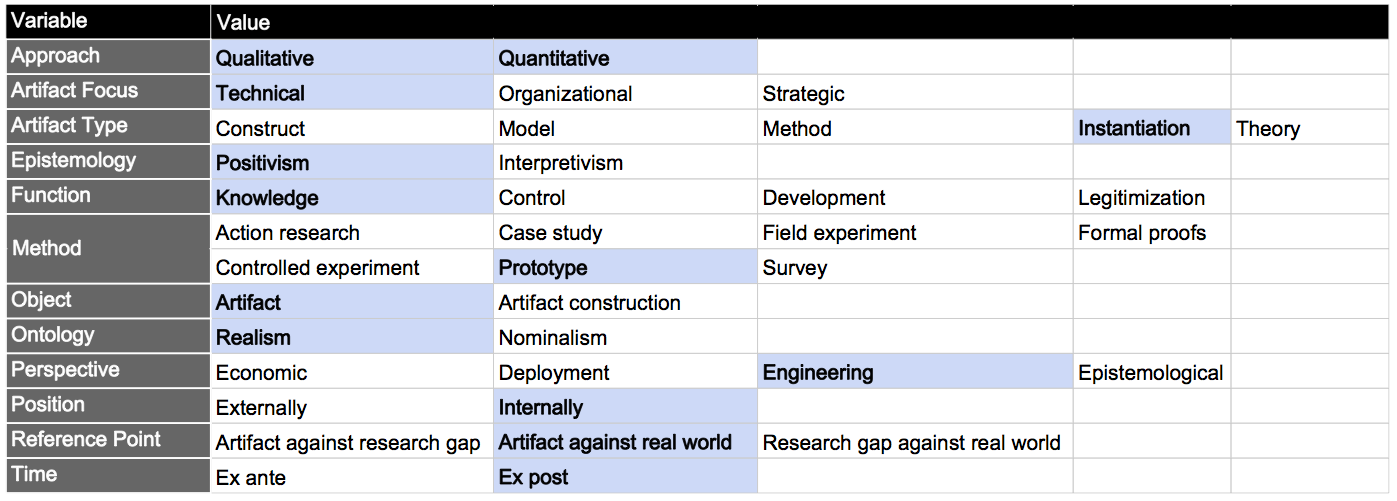
\includegraphics[width=0.7\pdfpagewidth]{figure/eval.png}
\caption{Evaluation matrix}
\label{fig:matrix}
\end{figure}

%This was done together with stakeholders at Ericsson. Once the problem was defined the solution objectives could then be inferred and delimited using the knowledge base to assess feasiblity. 

%Problem identification
%In this initial activity the specific research problem must be defined as it is used to inform the development of a solution and to justify it's value \cite{Peffers}.
%
%Objectives of a solution
%In this phase the goal is to infer solution objectives based on the problem definition while using the knowledgebase to assess feasibility \cite{Peffers}.
%
%Design and development
%In this activity, the wanted functionality of the artifact and it's architecture should be defined and the actual artifact should be developed.
%
%Demonstration
%Use the artifact to solve the identified problem. Many options exist for demonstration such as case studies, experimentation, simulation.
%
%Evaluation
%Solution objectives are compared to the observed results from the demonstration phase \cite{Peffers}. Use of relevant metrics and analysis techniques is important.
%
%Communication
%The problem and artifact should be clearly communicated to different audiences.

%-----------
%As  
%The evaluation of the artifacts are done both qualitatively and quantitatively. The   
%The artifacts will be evaluated both qualitatively and quantitatively. 
%
%
%
%%-----------
%
%
%\subsection{Data Collection}
%Data Collection
%\subsubsection{Qualitative}
%Interviews
%\subsubsection{Quantitative}
%Metrics
%*Size on disk comparing both against the relation database and comparing the different artifacts against each other.
%
%
%
%\subsection{Data Analysis}
%\subsubsection{Quantitative Data Analysis}
%\subsubsection{Qualitative Data Analysis}


%\section{Section levels}
%The following table presents an overview of the section levels that are used in this document. The number of levels that are numbered and included in the table of constants is set in the settings file \texttt{Settings.tex}. The levels are shown in Section \ref{Section_ref}.
%
%\begin{table}[h!]
%\centering
%\begin{tabular}{ll} \hline\hline
%Name & Command\\ \hline
%Section & \textbackslash\texttt{section\{\emph{Section name}\}}\\
%Subsection & \textbackslash\texttt{subsection\{\emph{Subsection name}\}}\\
%Subsubsection & \textbackslash\texttt{subsubsection\{\emph{Subsubsection name}\}}\\
%Paragraph & \textbackslash\texttt{paragraph\{\emph{Paragraph name}\}}\\
%Subparagraph & \textbackslash\texttt{paragraph\{\emph{Subparagraph name}\}}\\ \hline\hline
%\end{tabular}
%\end{table}
%
%\section{Section} \label{Section_ref}
%\subsection{Subsection}
%\subsubsection{Subsubsection}
%\paragraph{Paragraph}
%\subparagraph{Subparagraph}